\documentclass[12pt, twoside]{article}
\usepackage[francais]{babel}
\usepackage[T1]{fontenc}
\usepackage[latin1]{inputenc}
\usepackage[left=7mm, right=7mm, top=7mm, bottom=7mm]{geometry}
\usepackage{float}
\usepackage{graphicx}
\usepackage{array}
\usepackage{multirow}
\usepackage{amsmath,amssymb,mathrsfs} 
\usepackage{soul}
\usepackage{textcomp}
\usepackage{eurosym}
\usepackage{variations}
\usepackage{tabvar}


\begin{document}

\section*{\center{TD: Les fonctions affines}}

\ul{D�finition}: Une fonction affine est une fonction $f$ d�finie sur
$\mathbb{R}$ telle que $f(x)=ax+b$, $a$ et $b$ �tant deux r�els.

\enskip

La repr�sentation graphique d'une fonction affine $f(x)=ax+b$ est une 
\rule{3cm}{1pt}



$a$ est appell� \rule{8cm}{1pt}

\medskip

\begin{enumerate} 
  \item O� peut-on lire $b$?
  
  
  b est \rule{9cm}{1pt}
  
  \medskip
  
  \item Si $b=0$, que se passe-t-il? Comment appelle-t-on ce type de fonction?
  
  \rule{18cm}{1pt}
  
  \rule{18cm}{1pt}
  
 \medskip
 
  
  \item Si $a=0$, que se passe-t-il?
  
  
  \rule{18cm}{1pt}
  
  \rule{18cm}{1pt}
 
 \medskip
 
 
  \item Compl�ter les tableaux de variations et de signes : 
  % faire les tableaux de variations
  
  \begin{center}
  
  \textbf{Cas a>0}
  
  \medskip
  
\begin{tabular}{cc}


\begin{minipage}{8,5cm}



\renewcommand{\arraystretch}{2.5}
$\begin{array}{|c|ccccc|}
\hline
 x & -\infty & \  \ \ \ \ \ &  &\ \  \   \ \ &
 +\infty
 \\
 \hline
 f(x)=ax+b & \ \ &  & \ \ \ \ \ \ &  &
 \ \
 \\
 \hline
 \end{array}$

\end{minipage}

&

\begin{minipage}{8,5cm}




\enskip

\renewcommand{\arraystretch}{2.5}
$\begin{array}{|c|ccccc|}
\hline
 x & -\infty & \ \ \ \ \ \ & -\dfrac{b}{a} &\ \ \  \ \ \ &
 +\infty
 \\
 \hline
 f(x)=ax+b & \ \ & & \ \ \ \ \ \ \ &  &
 \ \
 \\
 \hline
 \end{array}$
\end{minipage}
\end{tabular}
\end{center}

\bigskip

\bigskip

  \begin{center}
  \textbf{Cas a<0}
  
  \medskip
  
\begin{tabular}{cc}

\begin{minipage}{8,5cm}





\enskip

\renewcommand{\arraystretch}{2.5}
$\begin{array}{|c|ccccc|}
\hline
 x & -\infty & \ \ \ \ \ \ &  &\ \ \ \  \ \ &
 +\infty
 \\
 \hline
 f(x)=ax+b & \ \ &  & \ \ \ \ \ \ \ &  &
 \ \
 \\
 \hline
 \end{array}$

\end{minipage}

&

\begin{minipage}{8,5cm}




\enskip

\renewcommand{\arraystretch}{2.5}
$\begin{array}{|c|ccccc|}
\hline
 x & -\infty & \ \ \ \ \ \ & -\dfrac{b}{a} &\ \ \ \ \ \ &
 +\infty
 \\
 \hline
 f(x)=ax+b & \ \ & & \ \ \ \ \ \ &  &
 \ \
 \\
 \hline
 \end{array}$
\end{minipage}
\end{tabular}
\end{center}
  
  \enskip
  
  \item Compl�ter le tableau en tra�ant dans chaques case une droite d'�quation $y=ax+b$.
  % faire les tableaux de variations
	\begin{center}
  		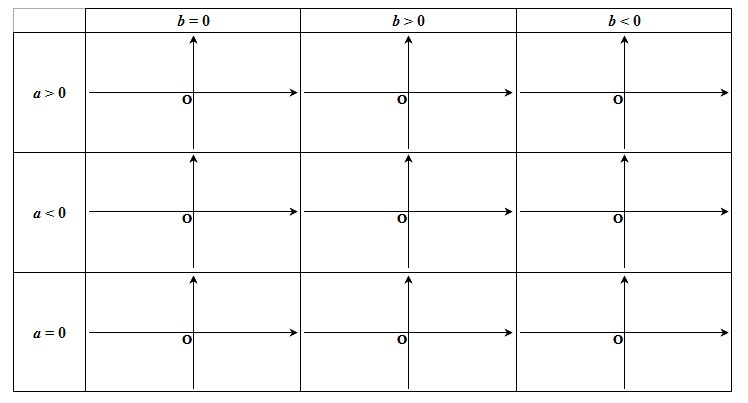
\includegraphics[width=14cm]{images/tableau1.jpg}
	\end{center}

\medskip


  \item Compl�ter:
  
  
	\begin{center}
  		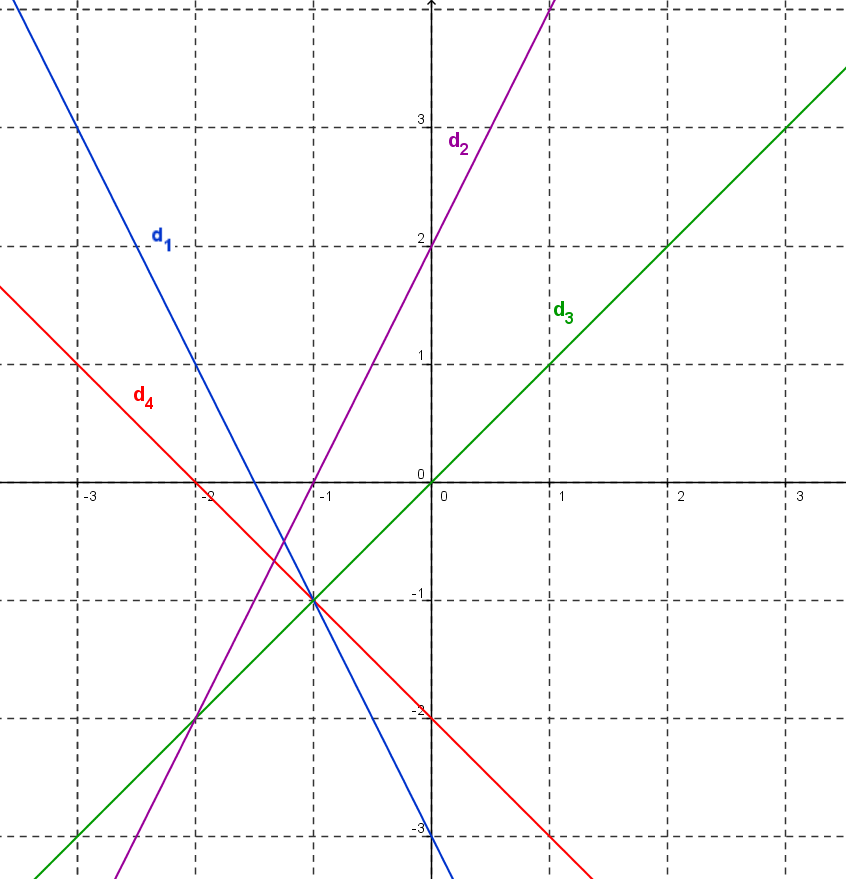
\includegraphics[width=12cm]{images/eq_droite.png}
  		
  		\medskip
  		
  		\bigskip
  		
  		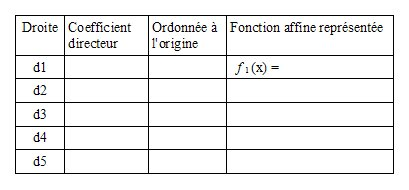
\includegraphics[width=12cm]{images/tableau.jpg}
	\end{center}
\end{enumerate}


\end{document}
